
\chapter{Description de l'API de \PpFf}
\label{description.chap}





\begin{figure}
\centering
     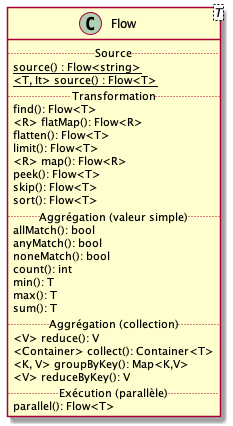
\includegraphics[scale=1.2]{Figures/flow-details.png}
      \caption{Les diff\'erentes m\'ethodes export\'ees par l'{API} de \ppff,
     regroup\'ees selon leur type de fonctionnalit\'e.}
       \label{MethodesAPI.fig}
\end{figure}


Ce chapitre pr\'esente l'API de la biblioth\`eque \ppff,  c'est-\`a-dire, l'interface avec laquelle interagit le d\'eveloppeur. La conception de l'API de \ppff{} permet aux utilisateurs de tirer parti de la simplicit\'e d'utilisation tout en cachant la complexit\'e des m\'ecanismes concurrents utilis\'es. La figure~\ref{MethodesAPI.fig} pr\'esente une vue d'ensemble des diverses m\'ethodes export\'ees par \ppff, exprimée à l'aide d'un diagramme de classes UML.%
%
\footnote{Tous les diagrammes de classes UML présentés dans ce mémoire ont été produits à l'aide de \TT{PlantUML}, un outil qui permet de spécifier un diagramme UML \emph{de fa\c{c}on textuelle} et qui génère ensuite, de façon automatique, le graphique correspondant, ici en format \TT{png}~: \url{https://plantuml.com/}.} 
%
Le type principal exporté par l'API est le type \TT{Flow}, qui permet de définir un \emph{flux de données} (Sect.~\ref{flow.sect}).
%
Ensuite, sur la base du type de fonctionnalit\'e export\'ee, l'API se divise en quatre cat\'egories :  \TT{Source} (Sect.~\ref{source.sect}), \TT{Transformation} (Sect.~\ref{transformation.sect}),  \TT{Agrégation} (Sect.~\ref{agregation.sect}) et \TT{Execution} (Sect.~\ref{execution.sect}). Quant \`a la cat\'egorie \TT{Agrégation}, elle est elle-m\^eme divis\'ee deux sous-cat\'egories, selon le type de r\'esultat produit~: valeur simple (par ex., r\'esultat bool\'een ou entier) ou collection.

L'objectif de notre API \'etait d'obtenir une API semblable \`a celle des \TT{Stream}s de \TT{Java}~8, bas\'ee sur le cha\^inage de m\'ethodes, donc la construction d'une séquence de traitements dans un style qui ressemble \`a un \TT{pipeline}.


Le chapitre pr\'esente \'egalement le code source d'un exemple, \TT{WordCount}, pour illustrer l'utilisation de l'API et l'effet des principales m\'ethodes --- un exemple semblable à celui présenté dans l'article ayant popularisé l'approche \TT{MapReduce}~\citep{DeanGhe04}.

La biblioth\`eque \PpFf{} est mise en \oe{}uvre au-dessus de la biblioth\`eque \TT{FastFlow}, mise en \oe{}uvre qui sera d\'ecrite au prochain chapitre.




\section{Exemple~: l'application \TT{WordCount}}
\label{descriptionWordCount.sect}


\begin{lstlisting}[
label={wordcount.c++},
language=c++,
caption={Des extraits du code source de l'application \TT{WordCount} qui compte le nombre d'occurrences des mots dans un texte.},
frame=single,
float]
    // Un conteneur pour les mots d'une ligne.
    typedef std::vector<std::string> Words;

    // Un Reducer pour combiner les elements.
    Reducer<std::string, int> reducer(
             0, 
             [](int count, std::string _) { return count + 1; },
             std::plus<int>{}
           );

    // Le resultat final, un map obtenu par traitement d'un flux.
    std::unordered_map<std::string, int> currentResult = 
        Flow
        ::source(inputFile)
        .parallel(4)
        .flatMap<std::string, Words, std::string>(splitInWords)			
        .map<std::string, std::string>(toLowercaseLetters)			
        .reduceByKey<std::string, std::string, int>(reducer); 
\end{lstlisting}

L'application \TT{WordCount} pr\'esent\'ee dans ce chapitre sera utilisée pour illustrer le fonctionnement de \TT{PpFf}. Des extraits du code source de l'application sont présentés dans le listing~\ref{wordcount.c++}. L'application compte le nombre d'occurrences des mots dans un fichier texte. Cette application est compos\'ee en combinant plusieurs op\'erations, qui forment le pipeline de traitement~:  

\begin{itemize}

\item  La premi\`ere op\'eration d'un pipeline sert \`a d\'efinir la \emph{source} du flux de donn\'ees. Ici, la source est
constitu\'ee par les lignes contenues dans un fichier. C'est la
m\'ethode statique \TT{source()} qui permet d'extraire et retourner un
flux avec les lignes du fichier. Le fichier est sp\'ecifi\'e par un nom de fichier
(une chaine, \TT{inputFile}) fourni en argument \`a la m\'ethode
\TT{source}.


\item L'appel \`a \TT{parallel(4)} permet de r\'epartir les \'el\'ements du flux entre divers \emph{threads} --- ici, quatre (4) instances de \emph{farm} --- et donc d'ex\'ecuter les \'etapes qui suivent en parall\`ele. 



\item L'op\'eration \TT{flatMap} d\'ecompose chaque ligne en mots individuels en appliquant la fonction \TT{splitInWords} sur chacune des lignes.

\item L'op\'eration \TT{map} transforme chacun des mots en rempla\c{c}ant les lettres majuscules d'un mot en lettres minuscules en appliquant la fonction \TT{toLowercaseLetters}.

\item Finalement, l'op\'eration \TT{reduceByKey}  regroupe les mots similaires ensemble et compte le nombre d'occurrences de chaque mot, et ce par l'utilisation du \TT{Reducer} (cf.~Sect.~\ref{reducer.sect}).
\end{itemize}


\section{Flux de donn\'ees: type \TT{Flow}}
\label{flow.sect}

L'interface de programmation propos\'ee par la bibliothèque \TT{PpFf} consiste en un ensemble de m\'ethodes qui permettent \`a l'utilisateur de manipuler des flux de donn\'ees de mani\`ere simple et efficace. L'interface s'inspire de celle introduite pour les \TT{Stream}s de \TT{Java} 8. L'annexe~\ref{methodes-api.ann} présente et d\'ecrit bri\`evement les m\'ethodes export\'ees par l'API, regroup\'ees selon leur fonctionnalit\'e, puis en ordre alphab\'etique \`a l'int\'erieur d'une cat\'egorie.



Comme on peut le voir dans le tableau de l'annexe~\ref{methodes-api.ann}, la d\'eclaration des m\'ethodes utilise la programmation \emph{g\'en\'erique} de C++, c'est-\`a-dire les \emph{templates}. Cela permet aux utilisateurs d'avoir une interface g\'en\'erique unique, de sorte qu'une m\'ethode peut \^etre r\'eutilis\'ee pour n'importe quel type de donn\'ees.


Un autre point cl\'e dans cette interface est son expressivit\'e. M\^eme avant sa conception d\'etaill\'ee, nous nous \'etions donn\'e comme objectif de fournir un syst\`eme suffisamment intuitif et expressif pour le traitement de flux de donn\'ees. Le cha\^inage de m\'ethodes et l'application d'expressions \emph{lambda} sont deux caract\'eristiques de \TT{PpFf} qui simplifient l'utilisation et facilitent la compr\'ehension du code.


\section{Cat\'egorie \TT{Source} : m\'ethodes \TT{source}}

\label{source.sect}

La sp\'ecification de la source de donn\'ees est la premi\`ere m\'ethode utilis\'ee pour cr\'eer un flux. Plus pr\'ecis\'ement, l'API fournit deux m\'ethodes {\bf statiques} pour cr\'eer un \TT{Flux} \`a partir de diverses sources, soit des collections ou des fichiers de donn\'ees. Des travaux futurs pourraient \'etendre l'interface pour prendre en charge plus des sources de donn\'ees.

Les signatures pour les deux m\'ethodes sont donn\'ees dans l'annexe~\ref{methodes-api.ann}. Tandis que la premi\`ere m\'ethode, \TT{source(path)}, produit les donn\'ees d'un flux \`a partir du contenu (les lignes) d'un fichier texte, la deuxi\`eme, \TT{source(begin\_iterator, end\_iterator)}, produit les donn\'ees d'un flux \`a partir des \'el\'ements d'un conteneur STL.

\begin{lstlisting}[
label={mapExample.c++},
language=c++,
caption={La transformation d'une collection d'entiers en une autre collection d'entiers en appliquant une expression lambda sur chacun des \'el\'ements.},
frame=single,
float]
std::vector<int> elems = {0, 1, 2, 3, 4, 5, 6, 7, 8, 9};

std::vector<int> currentResult =
  Flow::source<int>(elems.begin(), elems.end())
      .map<int, int>( [](int* in){ *in *= 3; return in; } )
      .collect<int, std::vector>();            
\end{lstlisting}

Les deux m\'ethodes pour sp\'ecifier la source d'un flux sont illustr\'ees, respectivement, dans les exemples des listings~\ref{wordcount.c++} et~\ref{mapExample.c++}. La m\'ethode \TT{source} du listing~\ref{wordcount.c++} envoie dans le flux chaque ligne du fichier. Le param\`etre \TT{inputFile} de la m\'ethode sp\'ecifie le chemin o\`u se trouve le fichier. Dans le deuxième exemple, celui du listing~\ref{mapExample.c++}, les donn\'ees sont consomm\'ees \`a partir de \TT{elems}, un \TT{vector}. La m\'ethode \TT{source} envoie dans le flux les donn\'ees de type \TT{int} du \TT{vector elems} en utilisant ses it\'erateurs de d\'ebut et fin.


\section{Cat\'egorie \TT{Transformation}}

\label{transformation.sect}

Cette section d\'ecrit plus en d\'etail les principales op\'erations de la cat\'egorie \TT{Transformation}. Ces op\'erations permettent d'exprimer des requ\^etes de traitement de donn\'ees complexes telles que le filtrage et le <<mappage>>. L'annexe~\ref{methodes-api.ann} présente les signatures détaillées de ces méthodes. 


\subsection{M\'ethode \TT{map}}



\begin{lstlisting}[
label={mapExample2.c++},
language=c++,
caption={La g\'en\'eration des noms de tous les employ\'es d'une collection dont le salaire est sup\'erieur \`a 1000.},
frame=single,
float]
std::vector<std::string> result =
  Flow::source<Employee>(elems.begin(), elems.end())
  	  .find<Employee>( [](Employee* e) -> bool 
					 { return e->salary > 1000; } )
      .map<Employee, std::string>( [](Employee* e) 
                                 { return &e->getName(); } )
      .collect<std::string, std::vector>();
\end{lstlisting}


La m\'ethode \TT{map} est utilis\'ee pour transformer une collection d'objets en une autre collection d'objets en appliquant une fonction --- typiquement une expression lambda --- sur chacun des objets. Par exemple, dans le listing~\ref{mapExample.c++}, l'expression lambda pass\'ee en param\`etre \`a la m\'ethode \TT{map} multiplie par 3 chaque \'el\'ement re\c{c}u. Le r\'esultat renvoy\'e par cette expression lambda est un pointeur. \PpFf{} s'appuie sur le mod\`ele de programmation de \TT{FastFlow}, tel que d\'ecrit dans le prochain chapitre. Ce mod\`ele est bas\'e sur le d\'ecouplage des donn\'ees et de la synchronisation, et o\`u seuls des pointeurs vers les donn\'ees sont transmis plut\^ot que les donn\'ees elles-m\^emes.
%
Une autre utilisation typique de la méthode \TT{map} consiste \`a obtenir une information de chacun des objets d'une collection. Par exemple, le listing~\ref{mapExample2.c++} montre un exemple o\`u la méthode \TT{map} permet d'obtenir les noms des divers employ\'es d'une collection. 


\subsection{M\'ethodes \TT{flatten} et \TT{flatMap}}

Les m\'ethodes \TT{flatten} et \TT{flatMap} ont pour r\^ole d'aplanir un flux multiniveau. Alors que la m\'ethode \TT{flatten} cr\'ee un flux unique \`a partir du contenu des divers conteneurs, la m\'ethode \TT{flatMap} cr\'ee un flux unique \`a partir du contenu des divers conteneurs interm\'ediaires r\'esultant de l'application d'une fonction fournie en argument et appliquée \`a chaque \'el\'ement du flux. Notons que cette derni\`ere m\'ethode (\TT{flatMap}) correspond en fait à une op\'eration \TT{map} suivie immédiatement d'une opération \TT{flatten}. Les signatures détaillées pour ces deux m\'ethodes sont donn\'ees dans l'annexe~\ref{methodes-api.ann}.

% Le type du flux avant d'appliquer les deux m\'ethodes est \TT{In} alors que \TT{Out} est le type du flux apr\`es le traitement des \'el\'ements du flux. 

Dans le cas de la m\'ethode \TT{flatMap}, le type \TT{Container} est le type interm\'ediaire r\'esultant de l'application de la fonction \TT{taskFunc} fournie en argument sur le flux. Par exemple, dans le listing~\ref{wordcount.c++}, \TT{Container} est de type \TT{Words} --- un vecteur de chaines de caract\`eres. Dans cet exemple, les lignes d'un fichier divis\'ees en mots sont accumul\'ees dans un conteneur et ensuite le contenu du conteneur est transmis sur le flux, un élément à la fois.


\subsection{M\'ethode \TT{find}}
Une op\'eration courante consiste \`a s\'electionner les \'el\'ements d'un ensemble de donn\'ees qui satisfont une certaine propri\'et\'e. L'API de \TT{PpFf} fournit une telle fonctionnalit\'e via la m\'ethode \TT{find}. Plus précisément, la m\'ethode \TT{find} s\'electionne les \'el\'ements d'un flux selon un pr\'edicat de sorte que seuls les \'el\'ements qui  satisfont le pr\'edicat sont envoy\'es \`a l'\'etape suivante. \`A noter qu'il est obligatoire que le pr\'edicat retourne une expression bool\'eenne. 

Un exemple qui illustre l'utilisation de la m\'ethode \TT{find} est pr\'esent\'e dans le listing~\ref{mapExample2.c++}~: l'appel \`a la m\'ethode \TT{find}  s\'electionne uniquement les employ\'es du flux dont le salaire est sup\'erieur \`a 1~000 \$.


\section{Cat\'egorie \TT{Agrégation}}

\label{agregation.sect}

La derni\`ere \'etape dans le traitement d'un flux est la collecte des \'el\'ements pour produire le r\'esultat. Les m\'ethodes fournies par l'API de la biblioth\`eque \ppff\ offrent quatre fonctionnalit\'es principales: 


\begin{itemize}
	\item Collecter les \'el\'ements du flux dans un conteneur;	

	\item R\'eduire les \'el\'ements de flux en une seule valeur;

	\item Regrouper les \'el\'ements selon une cl\'e;
	
	\item Regrouper les \'el\'ements selon une cl\'e et r\'eduire en une valeur associ\'ee.
\end{itemize}


\subsection{Collecte des \'el\'ements d'un flux dans un conteneur}

Afin de collecter les \'el\'ements d'un flux dans un conteneur, l'{API} de \TT{PpFf} fournit la m\'ethode \TT{collect}. Cette m\'ethode retourne un conteneur {STL}. Le type pour les \'el\'ements du conteneur et le type du conteneur sont donn\'es par les types indiqu\'es en param\`etres \emph{template} de la m\'ethode \TT{collect}. 

L'exemple fourni dans le listing~\ref{mapExample2.c++} montre l'utilisation de la m\'ethode \TT{collect}. La m\'ethode collecte les noms des employ\'es d'une collection d'\TT{Employee}s dans un \TT{vector} de \TT{string}s.


\subsection{R\'eduction des \'el\'ements d'un flux en une seule valeur}


\begin{lstlisting}[
label={olderEmployeeExample.c++},
gobble=4,
language=c++,
caption={Un pipeline pour identifier l'employ\'e le plus ag\'e.},
frame=single,
float]
    Employee currentResult = 
      Flow::source<Employee>(employees.begin(), employees.end())
          .parallel(4)
          .max<Employee>( [](Employee* older, Employee* e) 
                          { if (e->age > older->age) *older = *e; } );
\end{lstlisting}


Une r\'eduction
consiste \`a combiner les \'el\'ements d'un flux en un seul r\'esultat \emph{qui n'est pas un flux}. La m\'ethode \TT{max}  est l'une des m\'ethodes offertes par l'{API} de \TT{PpFf} qui illustre ce type de fonctionnalit\'e. Cette m\'ethode prend un comparateur en argument pour comparer les \'el\'ements du flux. 
%
Le listing~\ref{olderEmployeeExample.c++} montre un exemple o\`u les \'el\'ements de type \TT{Employee} d'un flux sont compar\'es afin de trouver l'employ\'e le plus \^ag\'e.


De façon similaire \`a la m\'ethode \TT{max}, l’API de \TT{PpFf} fournit aussi la m\'ethode \TT{min}, utilis\'ee pour trouver l'\'el\'ement minimum d'un flux. Ceci est fait en utilisant le comparateur re\c{c}u comme argument pour comparer les \'el\'ements du flux.

L'{API} fournit d'autres m\'ethodes qui r\'eduisent les \'el\'ements d'un flux \`a une seule valeur. Parmi les plus simples on trouve \TT{count} et \TT{sum}. En utilisant \TT{count}, on obtient le nombre d'\'el\'ements d'un flux, alors qu'en utilisant \TT{sum}, on additionne les \'el\'ements d'un flux. Une autre m\'ethode plus g\'en\'erale fournie par l'{API} de \TT{PpFf} est \TT{reduce}, qui \emph{combine} les \'el\'ements d'un flux en utilisant un \TT{Reducer}, notion pr\'esent\'ee dans la section suivante.


\subsection{Classe \TT{Reducer}}

\label{reducer.sect}

La m\'ethode \TT{reduce} est l'une des m\'ethodes les plus complexes de l'API. Afin de r\'eduire les \'el\'ements d'une collection \`a une seule valeur, la m\'ethode \TT{reduce} doit couvrir quatre cas distincts : 

\begin{itemize}
\item R\'eduire les \'el\'ements d'une collection sans spécifier de valeur initiale~; 

\item R\'eduire les \'el\'ements d'une collection \`a partir d'une valeur initiale fournie par l'utilisateur~; 

\item R\'eduire les \'el\'ements d'une collection en parall\`ele sans spécifier de valeur initiale~; 

\item R\'eduire les \'el\'ements d'une collection en parall\`ele \`a partir d'une valeur initiale fournie par l'utilisateur.
\end{itemize}

Pour impl\'ementer tous ces cas nous aurions d\^u surcharger la m\'ethode  \TT{reduce} plusieurs fois. Dans le but de garder une API simple \`a utiliser, nous avons introduit la classe  \TT{Reducer}. Cette classe est d'autant plus utile que sa fonctionnalit\'e est r\'eutilis\'ee dans d'autres m\'ethodes de l'API --- voir la section~\ref{reduceByKey.sect}


\begin{lstlisting}[
label={reducer.c++},
gobble=1,
language=c++,
caption={La signature de la classe \TT{Reducer} avec ses quatre constructeurs.},
frame=single,
float]
 template<typename In, typename Out>
 class Reducer {
     Reducer(std::function<Out(Out, In)> const& accumulator);

     Reducer(Out initialValue, 
             std::function<Out(Out, In)> const& accumulator);
                	   
     Reducer(std::function<Out(Out, In)> const& accumulator,
             std::function<Out(Out, Out)> const& combiner);
                               	   
     Reducer(Out initialValue, 
             std::function<Out(Out, In)> const& accumulator,
             std::function<Out(Out, Out)> const& combiner);               
 }
\end{lstlisting}


Un objet de la classe \TT{Reducer} est utilis\'e pour sp\'ecifier comment r\'eduire les \'el\'ements d'un flux \`a une valeur unique. Le listing~\ref{reducer.c++} présente la spécification  de la classe \TT{Reducer} avec les signatures des quatre constructeurs associ\'es. 

Un \TT{Reducer} peut être construit avec une valeur initiale, une fonction \TT{accumulator} et une fonction \TT{combiner}. La valeur initiale et la fonction \TT{combiner} sont optionnelles.%
%
\footnote{Notons que si la valeur initiale n'est pas spécifiée, alors
c'est le premier élément du flux qui est utilisée pour initialiser
l'accumulateur, et donc le flux doit contenir \emph{au moins un élément} pour
qu'un résultat puisse être produit.}
%
Les constructeurs de \TT{Reducer} permettent de fournir la fonctionnalit\'e de la m\'ethode \TT{reduce} en couvrant les quatre cas distincts mentionn\'es au d\'ebut de la section.
%


\begin{lstlisting}[
language=c++,
label={olderEmployeeWithReduceExample.c++},
caption={Un autre pipeline pour identifier l'employ\'e le plus ag\'e, mais avec un \TT{Reducer} et sans parallélisme.},
frame=single,
gobble=4,
escapechar=\!,
float]
    Reducer<Employee, Employee> 
           reduceAgeMax( [](Employee e1, Employee e2) 
                         { return e1.age > e2.age !?! e1 : e2; } );

    Employee currentResult =
        Flow::source<Employee>(employees.begin(), employees.end())
            .reduce<Employee, Employee>(reduceAgeMax);
\end{lstlisting}


La fonction \TT{accumulator} est utilis\'ee pour effectuer l'op\'eration de r\'eduction sur les éléments du flux. Cette fonction prend deux paramàtres: le premier est le r\'esultat partiel de l'op\'eration de r\'eduction  --- la valeur de l'accumulateur --- et le deuxi\`eme est l'\`el\'ement suivant du flux. Par exemple, le listing~\ref{olderEmployeeWithReduceExample.c++} montre l'exemple du listing~\ref{olderEmployeeExample.c++}, mais r\'e\'ecrit avec la m\'ethode \TT{reduce} et un \TT{Reducer}. Le constructeur de la classe \TT{Reduce} prend comme argument la fonction \TT{accumulator} tout en ignorant la valeur initiale est la fonction \TT{combiner}. La fonction \TT{accumulator} effectue l'op\'eration de r\'eduction en trouvant l'employ\'e le plus \^ag\'e. 


\begin{lstlisting}[
label={sumElementsCollectionWithReducerParallel.c++},
gobble=4,
language=c++,
caption={[Un exemple d'utilisation d'un \TT{Reducer}, ex\'ecut\'e en
parall\`ele et avec une valeur initiale.]Un exemple
d'utilisation d'un \TT{Reducer}, ex\'ecut\'e en parall\`ele et avec une
valeur initiale sp\'ecifi\'ee explicitement.},
frame=single,
float]
    int n = 100;
    std::vector<int> elems(n);
    for (unsigned int i = 0; i < elems.size(); i++) {
        elems[i] = i;
    };

    // Avec valeur initiale explicite... pour illustrer l'effet!
    Reducer<int, int> reducer(3, 
                              std::plus<int>{}, 
                              std::plus<int>{});

	int currentResult =
		Flow::source<int>(elems.begin(), elems.end())
            .parallel(2)
            .reduce<int, int>(reducer); 
	
	std::cout << "Result: " << currentResult;	// == 4953
\end{lstlisting}


Le troisi\`eme param\`etre du constructeur d'un \TT{Reducer}, la fonction \TT{combiner}, est utilis\'e lorsque le flux est trait\'e en parall\`ele, en utilisant les instances parall\`eles d'un \emph{farm}. Dans un tel cas, le flux est divis\'e en sous-flux --- i.e., chaque instance d'un \emph{farm} traite un sous-ensembles des éléments --- qui sont r\'eduits en parall\`ele avec la fonction \TT{accumulator}. Les r\'esultats partiels produits par les diverses instances d'un \emph{farm} sont ensuite combin\'es, dans le \emph{thread} principal, avec la fonction \TT{combiner}. Le listing~\ref{sumElementsCollectionWithReducerParallel.c++} montre un exemple d'utilisation d'un \TT{Reducer} mais ex\'ecut\'e en parall\`ele. Dans cet exemple, \`a des fins d'illustration, une valeur initiale est sp\'ecifi\'ee, \'egale \`a \TT3, alors que les fonctions \TT{combiner} et \TT{accumulator} sont toutes deux indiqu\'ees explicitement comme \'etant la fonction d'addition \TT{std::plus<int>\{\}}. 


\begin{lstlisting}[
label={sumElementsCollectionParallelWithoutCombiner.c++},
gobble=4,
language=c++,
caption={[Un exemple d'ex\'ecution en parall\`ele de la m\'ethode \TT{reduce}]Un exemple d'ex\'ecution en parall\`ele de la m\'ethode \TT{reduce} sans utiliser la fonction \TT{combiner}.},
frame=single,
float]
    int n = 100;
    std::vector<int> elems(n);
    for (unsigned int i = 0; i < elems.size(); i++) {
        elems[i] = i;
    };

	int currentResult =
		Flow::source<int>(elems.begin(), elems.end())
            .parallel(2)
            .reduce<int, int>(3, std::plus<int>{}); 
	
	std::cout << "Result: " << currentResult;	// == 4953
\end{lstlisting}



Il existe des situations o\`u la fonction \TT{accumulator} est identique à la fonction \TT{combiner}, par exemple, celui illustr\'e dans le listing~\ref{sumElementsCollectionWithReducerParallel.c++}. L'API de \TT{PpFf} fournit une surcharge de la m\'ethode \TT{reduce} pour pouvoir omettre la fonction \TT{combiner} m\^eme si l'ex\'ecution est en parall\`ele. Le listing~\ref{sumElementsCollectionParallelWithoutCombiner.c++} montre l'exemple du listing~\ref{sumElementsCollectionWithReducerParallel.c++}, mais r\'e\'ecrit en omettant la fonction \TT{combiner}. 




La description (semi-)formelle d'un \TT{Reducer} --- d\'ecrite par mon directeur de recherche --- est pr\'esent\'ee dans l'annexe~\ref{DescriptionFormelleReducer.ann}.



\subsection{Regroupement des \'el\'ements selon une cl\'e}

Souvent, une op\'eration sur une collection de donn\'ees consiste \`a regrouper ses \'el\'ements dans un ensemble en fonction d'une ou plusieurs propri\'et\'es. Notre {API} fournit une fonctionnalit\'e similaire via la m\'ethode \TT{groupByKey}.


\begin{lstlisting}[
label={groupByKeyExample.c++},
escapechar=\!,
language=c++,
caption={[Un pipeline pour regrouper les employ\'es selon leur \^age.]Un pipeline pour regrouper les employ\'es selon leur \^age.\ExtraitTestUnitaire},
frame=single,
float]
typedef std::unordered_map<int, std::vector<Employee>> 
        EMPLOYES_PAR_AGE;

// Definition (omise) d'un vecteur d'objets Employee.
std::vector<Employee> employees = ...; 
employees[3].age = employees[4].age = 18;
employees[0].age = employees[1].age = employees[2].age = 22;
employees[7].age = employees[8].age = 33;
employees[5].age = employees[6].age = employees[9].age = 55;

EMPLOYES_PAR_AGE result = 
   Flow::source<Employee>(employees.begin(), employees.end())
       .groupByKey<Employee, int, Employee>( // Regroupe selon l'age.
           [](Employee* e) { return &e->age; } 
        );
    
EMPLOYES_PAR_AGE expected = {
   {18, {employees[3], employees[4]}},
   {22, {employees[0], employees[1], employees[2]}},
   {33, {employees[7], employees[8]}},
   {55, {employees[5], employees[6], employees[9]}}
};

// !\emph{Assertions (omises) qui montrent que \TT{result} d\'enote}!
// !\emph{un map \'equivalent \`a celui repr\'esent\'e par \TT{expected}!}!
  ...
\end{lstlisting}




Le listing~\ref{groupByKeyExample.c++} montre un exemple o\`u les employ\'es sont regroup\'es selon leur \^age. Plus pr\'ecis\'ement, ce listing pr\'esente un des tests unitaires pour \TT{groupByKey}, qui montre que les employ\'es d'un conteneur sont regroup\'es dans un \TT{map} o\`u la cl\'e est l'\^age des employ\'es et la valeur est un \TT{vector} contenant les employ\'es de m\^eme \^age.
%

\begin{lstlisting}[
label={groupByKeyExample2.c++},
escapechar=\!,
language=c++,
caption={[Un pipeline pour regrouper les noms d'employ\'es selon leur \^age.]Un pipeline pour regrouper les noms d'employ\'es selon leur \^age.\ExtraitTestUnitaire},
frame=single,
float]
typedef std::unordered_map<int, std::vector<std::string>> 
        NOMS_EMPLOYES_PAR_AGE;

// Definition (omise) d'un vecteur d'objets Employee 
// ou le nom de employes[0] est "Employee0", etc.
std::vector<Employee> employees = ...; 
employees[3].age = employees[4].age = 18;
employees[0].age = employees[1].age = employees[2].age = 22;
employees[7].age = employees[8].age = 33;
employees[5].age = employees[6].age = employees[9].age = 55;

NOMS_EMPLOYES_PAR_AGE result = 
   Flow::source<Employee>(employees.begin(), employees.end())
       .groupByKey<Employee, int, std::string>(
          [](Employee* e) { return &e->age; },
          [](Employee* e) { return &e->name; }
       );
    
NOMS_EMPLOYES_PAR_AGE expected = {
   {18, {"Employee3", "Employee4"}},
   {22, {"Employee0", "Employee1", "Employee2"}},
   {33, {"Employee7", "Employee8"}},
   {55, {"Employee5", "Employee6", "Employee9"}}
};

// !\emph{Assertions (omises) qui montrent que \TT{result} d\'enote}!
// !\emph{un map \'equivalent \`a celui repr\'esent\'e par \TT{expected}!}!
  ...
\end{lstlisting}


La m\'ethode \TT{groupByKey} comporte en fait deux param\`etres, mais le deuxi\`eme param\`etre est optionnel. Ce param\`etre est une fonction qui s'applique sur les \'el\'ements s\'electionn\'es pour produire les \'el\'ements du \TT{map}. Par exemple,  le listing~\ref{groupByKeyExample2.c++} pr\'esente presque le m\^eme exemple que dans le listing~\ref{groupByKeyExample.c++}, o\`u les employ\'es sont regroup\'es selon leur \^age, mais dans ce deuxi\`eme cas, la valeur r\'esultante ajout\'ee au conteneur est le nom de l'employ\'e --- et non l'employ\'e lui-m\^eme. On obtient donc un \TT{map} o\`u la cl\'e est un \^age et la valeur est un \TT{vector} \emph{des noms d'employ\'es} ayant cet \^age --- et non un \TT{vector} des employ\'es.


La description (semi-)formelle de \TT{groupByKey} --- d\'ecrite par mon directeur de recherche --- est pr\'esent\'ee dans l'annexe~\ref{DescriptionFormelleGroupByKey.ann}.




\subsection{Regroupement des \'el\'ements selon une cl\'e et r\'eduction d'une valeur associ\'ee}

\label{reduceByKey.sect}

\begin{lstlisting}[
label={reduceByKeyExample.c++},
escapechar=\!,
language=c++,
caption={[Un pipeline pour compter le nombre d'employ\'es de chaque \^age.]Un pipeline pour compter le nombre d'employ\'es de chaque \^age.\ExtraitTestUnitaire},
frame=single,
float]
typedef std::unordered_map<int, int> NO_EMPLOYES_PAR_AGE;

// Definition (omise) d'un vecteur d'objets Employee.
std::vector<Employee> employees = ...; 
employees[3].age = employees[4].age = 18;
employees[0].age = employees[1].age = employees[2].age = 22;
employees[7].age = employees[8].age = 33;
employees[5].age = employees[6].age = employees[9].age = 55;

Reducer<Employee, int> reducer(
      0,
      [](int count, Employee _) { return count + 1; }
    );

NB_EMPLOYES_PAR_AGE result = 
   Flow::source<Employee>(employees.begin(), employees.end())
       .reduceByKey<Employee, int, int>(
             reducer, [](Employee* e) { return &e->age; }
     );
    
NB_EMPLOYES_PAR_AGE expected = {
   {18, 2},
   {22, 3},
   {33, 2},
   {44, 1},
   {55, 2}
};

// !\emph{Assertions (omises) qui montrent que \TT{result} d\'enote}!
// !\emph{un map \'equivalent \`a celui repr\'esent\'e par \TT{expected}!}!
  ...
\end{lstlisting}

Une op\'eration de regroupement et r\'eduction peut \^etre verbeuse et source d'erreurs lorsqu'elle est impl\'ement\'ee dans un style imp\'eratif. L'{API} fournit une fonction qui combine ces deux op\'erations, et ce  dans un style fonctionnel~: la m\'ethode \TT{reduceByKey}.

Le listing~\ref{reduceByKeyExample.c++} montre un exemple o\`u une telle fonctionnalit\'e est utile. Le listing pr\'esente un des tests unitaires pour \TT{reduceByKey}, qui d\'enombre les employ\'es en fonction de leur cat\'egorie d'\^age. 

La m\'ethode \TT{reduceByKey} conserve les \'el\'ements dans un conteneur de type cl\'e--valeur --- donc un dictionnaire (\TT{map}). La cl\'e de chaque \'el\'ement du flux est cherch\'ee dans le conteneur. Si la cl\'e n'est pas trouv\'ee, une nouvelle paire cl\'e--valeur est ajout\'ee. Si la cl\'e est trouv\'ee, la fonction de r\'eduction est appliqu\'ee sur l'\'el\'ement du flux et sa valeur associ\'ee dans le conteneur. L'op\'eration de r\'eduction --- un objet \TT{Reducer} (section~\ref{reducer.sect})  --- est sp\'ecifi\'ee par l'argument de la m\'ethode \TT{reduceByKey}. Dans le cas particulier de l'exemple fourni dans le listing~\ref{reduceByKeyExample.c++}, l'op\'eration a pour r\^ole de compter le nombre d'employ\'es ayant le m\^eme \^age. Le r\'esultat retourn\'e par la m\'ethode \TT{reduceByKey} est un map de type cl\'e--valeur~: la cl\'e repr\'esente l'\^age d'employ\'es et la valeur associ\'ee repr\'esente le nombre d'employ\'es qui ont l'\^age indiqu\'e par la cl\'e.

La m\'ethode \TT{reduceByKey} est une op\'eration avec une mise en \oe{}uvre complexe, encore plus lorsqu'elle est utilis\'ee en parall\`ele. Toutefois, la biblioth\`eque \TT{PpFf} cache cette complexit\'e, et donc il est tout à fait possible et intéressant d'utiliser \TT{reduceByKey} en parall\`ele, et dans ce cas le temps d'ex\'ecution peut être réduit --- sous certaines conditions que nous examinerons au chapitre~\ref{experiences.chap}.


Lorsque le flux est trait\'e en parall\`ele, il est divis\`e en sous-flux. Chaque instance cr\'ee et manipule son propre \emph{container}, son propre \emph{map}, donc sans interf\'erence avec les \emph{threads} qui traitent les autres sous-flux. Puis, lors de la combinaison des r\'esultats des sous-flux, ces divers \emph{containers/maps} sont fusionn\'es les uns avec les autres dans le \emph{thread} principal.


\section{Cat\'egorie \TT{Execution}}

\label{execution.sect}


Dans \TT{PpFf}, par d\'efaut, chaque nœud ajout\'e dans le flux du traitement s'ex\'ecute sur un \emph{thread} diff\'erent. En plus, la biblioth\`eque \TT{PpFf} permet d'introduire aussi du parall\'elisme de données, par le biais d'instances de \emph{farm}. Ces instances sont cr\'e\'ees en appelant la m\'ethode \TT{parallel} de l’API.  

La méthode \TT{parallel} reçoit un argument entier.
%
La valeur de cet argument permet de sp\'ecifier le nombre d'instances parall\`eles d'un \emph{farm} entre lesquelles seront r\'epartis les \'el\'ements du flux \`a traiter. Par exemple, dans le listing~\ref{wordcount.c++}, l'appel \`a la m\'ethode \TT{parallel(4)} indique de r\'epartir les \'el\'ements du flux entre quatre (4) instances parall\`eles d'un \emph{farm}.



\section{Expressivit\'e de \TT{PpFf} par rapport à \TT{FastFlow} et
\TT{Java}}

\GT{Ajouter ici quelques mots d'introduction.}

\label{PpFfExpressivities.sect}




\subsection{\texttt{PpFf} vs.\ \texttt{FastFlow}}


\'Ecrit au-dessus de la biblioth\`eque \TT{FastFlow}, \TT{PpFf} essaie de simplifier le traitement des collections de donn\'ees par rapport à \TT{FastFlow}. Dans ce qui suit, à l'aide d'exemples simples, nous pr\'esenterons ce qui distingue \ppff\ de \TT{FastFlow}.



\subsection*{Chainage de m\'ethodes et expressions \emph{lambda}}

\begin{lstlisting}[
label={FastFlowOperationsToGroupStudentsByDep.c++},
language=c++,
caption={[a)~Les op\'erations auxiliaires utilisées par un pipeline \TT{FastFlow}.]a)~Les op\'erations auxiliaires utilisées par le pipeline \TT{FastFlow} du listing~\ref{GroupByDepStudentsAverageFF.c++}~b), qui vise à regrouper les \'etudiants boursiers par d\'epartement.},
frame=single,
float]
    // Premiere operation dans le flux = source de donnees.
	struct source : ff_node {
		Students students;
		source(Students students) : students(students){}
		void* svc(void*) {
			for (auto &elem: students) {
				ff_send_out(&elem);
			}	
			return EOS;	
		}
	};
	// Operation de filtrage pour les etudiants boursiers.
	struct findStudentsAverage : ff_node_t<Student, Student> {
		Student* svc(Student* task) {
			if (task->average == "A") {
				return task;
			}
			return GO_ON;
		}
	};
	// Operation de regroupement des etudiants par departement.
	struct groupByDepartement : ff_node_t<Student, void> {
		Students_by_Dept& container;
		groupByDepartement(Students_by_Dept& container) :
									container(container){}
		void* svc(Student* task) {
			auto mapIt = container.find(task->departement);
			if (mapIt != container.end()) {
				mapIt->second.push_back(*task);
			} else {
				Students students = {*task};
				container[task->departement] = students;
			}
			return GO_ON;		
		}
	};      
\end{lstlisting}


\addtocounter{lstlisting}{-1}

\begin{lstlisting}[
label={GroupByDepStudentsAverageFF.c++},
language=c++,
caption={[b)~Un pipeline \TT{FastFlow} pour regrouper les \'etudiants boursiers par d\'epartement.]b)~Un pipeline \TT{FastFlow} pour regrouper les \'etudiants boursiers par d\'epartement. Les op\'erations auxiliaires utilisées par le pipeline sont d\'efinies dans le listing~\ref{FastFlowOperationsToGroupStudentsByDep.c++}~a).\ExtraitTestUnitaire},
frame=single,
float]

	// Conteneur pour le resultat du traitement.
	Students_by_Dept result;
	// Creation du pipeline.
	ff_Pipe<> ffp( new source(students),
				   new findStudentsAverage,
				   new groupByDepartement(result) );        

\end{lstlisting}

\TT{FastFlow} est une biblioth\`eque de bas niveau pour traiter des collections et flux de donn\'ees. Travailler avec des collections n'est pas toujours facile lorsque, comme en \TT{FastFlow}, le traitement doit être décrit en indiquant explicitement, pour chaque élément du flux,  soit le ou les nouveaux éléments à émettre sur le flux (\TT{ff\_send\_out(\ldots)} ou \TT{return task}), soit le fait que le traitement de l'élément ne produit aucun résultat (\TT{return GO\_ON})

Par exemple, supposons que dans une universit\'e, on doit identifier les \'etudiants boursiers ayant une moyenne de \TT{A}, puis les regrouper par d\'epartement.

\goodbreak
\begin{samepage}
Supposons aussi qu'on ait les types auxiliaires suivants~:
\begin{lstlisting}[language=c++]
    // Nom d'un departement.
    typedef std::string Dept;
    
    // Conteneur pour les etudiants d'un meme departement.
    typedef std::vector<Student> Students;

    // Conteneur pour regrouper les etudiants par departement.
    typedef std::unordered_map<Dept, Students> Students_by_Dept; 
\end{lstlisting}
\end{samepage}


Les listings~\ref{FastFlowOperationsToGroupStudentsByDep.c++}~a) et \ref{GroupByDepStudentsAverageFF.c++}~b) montrent un exemple de solution avec un pipeline \TT{FastFlow} pour ce problème. Le listing~\ref{FastFlowOperationsToGroupStudentsByDep.c++}~a) contient les définitions des opérations requises pour créer le flux. La création du flux est illustrée dans le listing~\ref{GroupByDepStudentsAverageFF.c++}~b). On peut observer que pour chaque op\'eration dans le flux, on doit définir une nouvelle fonction qui traite chaque élément. De plus, il est difficile de comprendre d'un coup d'œil ce que fait le code: les op\'erations sont d'abord d\'efinies dans diff\'erents nœuds (\TT{struct} de type \TT{ff\_node} ou \TT{ff\_node\_t}) et sont ensuite utilis\'ees dans la cr\'eation du flux. 

\begin{lstlisting}[
label={GroupByDepStudentsAverage.c++},
language=c++,
caption={[Un pipeline \ppff\ pour regrouper les \'etudiants boursiers par d\'epartement.]Un pipeline \ppff\ pour regrouper les \'etudiants boursiers par d\'epartement.\ExtraitTestUnitaire},
frame=single,
float]
    // Resultat du traitement.
    Students_by_Dept result = 
        Flow
        ::source<Student>(students.begin(), students.end())
        .find<Student>( [](Student *s) { return s->average == "A"; } )
        .groupByKey<Student, Dept, Student>(
            [](Student* s) { return &(s->departement); } );        
\end{lstlisting}

Avec \TT{PpFf}, ce probl\`eme peut \^etre r\'esolu plus simplement en utilisant le chainage de m\'ethodes et des expressions \emph{lambda}. \TT{PpFf} propose de nombreuses m\'ethodes pr\'ed\'efinies pour les op\'erations de traitement de flux les plus utilis\'ees. Le listing~\ref{GroupByDepStudentsAverage.c++} montre l'exemple du listing~\ref{GroupByDepStudentsAverageFF.c++}, mais r\'e\'ecrit avec \TT{PpFf}. On peut noter que le code est plus facile \`a comprendre. Les op\'erations sont définies \`a la cr\'eation du flux. De plus, le nombre de lignes de code utilis\'e dans la version \TT{PpFf} est consid\'erablement r\'eduit comparativement \`a \TT{FastFlow}. 

Le principal avantage de l'utilisation du chainage de m\'ethodes est donc que le code est plus lisible, et les op\'erations à exécuter sont pass\'ees au flux sous forme de blocs d'instructions, et ce avec des expressions \emph{lambda}.
%
De plus, avec \TT{find}, il n'est pas nécessaire de traiter l'envoi de
signaux (\TT{return GO\_ON}) lorsqu'un élément ne satisfait pas une
condition, donc ne produit pas d'élément à la sortie du flux.


%\subsection*{Expressions \emph{lambda}}


L'utilisation d'expressions \emph{lambda} permet, entre autres, de
facilement changer le traitement effectué par une opération d'un
pipeline.
%
Par exemple, prenons l'exemple du listing~\ref{GroupByDepStudentsAverageFF.c++} o\`u on sélectionne les \'etudiants boursiers ayant une moyenne de \TT{A}. Que se passe-t-il si on veut plutôt sélectionner les \'etudiants qui habitent dans une certaine ville? Dans \TT{FastFlow}, une solution serait d'impl\'ementer une nouvelle sorte de nœud et d'utiliser ce n\oe{}ud dans la cr\'eation d'un flux. 
%
Il est un peu ennuyeux d'avoir \`a \'ecrire beaucoup de code pour des fonctionnalit\'es simples lorsqu'elles ne sont peut-\^etre utilis\'ees qu'une ou deux fois. Id\'ealement, on souhaite minimiser les efforts de d\'eveloppeurs et offrir des op\'erations simples \`a mettre en œuvre.


\TT{PpFf} offre la possibilit\'e d'utiliser des expressions \emph{lambda} directement dans la cr\'eation du flux.
%
Ici, il suffirait donc de modifier l'appel à \TT{find} comme suit lors de la création du pipeline pour sélectionner les étudiants provenant de Montréal~: 
{
\begin{lstlisting}[language=c++]
		.find<Student>( 
			[](Student *s) { s->city_address == "Montreal"; } )
\end{lstlisting}
}


\subsection*{Traitement en parall\`ele}

De nos jours, tous les nouveaux ordinateurs sont des ordinateurs multicœurs. Au lieu d'un seul processeur, ils en disposent de plusieurs. Les deux biblioth\`eques, \TT{FastFlow} et \TT{PpFf}, peuvent am\'eliorer le traitement des grandes collections de donn\'ees si les ressources d'une telle machine peuvent être exploitées efficacement. 

\begin{lstlisting}[
label={GroupByDepStudentsAverageParallelFF.c++},
language=c++,
caption={[Un pipeline \TT{FastFlow} pour regrouper les \'etudiants boursiers par d\'epartement en utilisant les instances parall\`eles d'un \emph{farm}.]Un pipeline \TT{FastFlow} pour regrouper les \'etudiants boursiers par d\'epartement en utilisant les instances parall\`eles d'un \emph{farm}.\ExtraitTestUnitaire},
frame=single,
float]
	// Creation des instances de travailleurs d'un farm.
	std::vector<ff_node*> workers;
	for ( uint32_t i = 0; i < PAR_LEVEL; i++ ) {
		workers.push_back( new ff_Pipe<>(new findStudentsAverage) );
	}

	Students_by_Dept result;
	ff_Pipe<> ffp( new source(students),
				   new ff_farm(workers),
				   new groupByDepartement(result) );     
\end{lstlisting}

\begin{lstlisting}[
label={GroupByDepStudentsAverageParallel.c++},
language=c++,
caption={[Un pipeline \ppff\ pour regrouper les \'etudiants boursiers par d\'epartement en utilisant les instances parall\`eles d'un \emph{farm}.]Un pipeline \ppff\ pour regrouper les \'etudiants boursiers par d\'epartement en utilisant les instances parall\`eles d'un \emph{farm}.\ExtraitTestUnitaire},
frame=single,
float]
    Students_by_Dept result = 
        Flow
        ::source<Student>(students.begin(), students.end())
        .parallel(PAR_LEVEL) // Ajout simple d'un appel a parallel
        .find<Student>( [](Student *s) { return s->average == "A"; } )
        .groupByKey<Student, Dept, Student>(
           [](Student* s) { return &(s->departement); } );
\end{lstlisting}

Par d\'efaut, chaque nœud d'un flux dans \TT{FastFlow} et \TT{PpFf} s'ex\'ecute dans un \emph{thread} diff\'erent. Le traitement d'un flux peut \^etre davantage parall\'elis\'e si on utilise aussi les instances parall\`eles d'un \emph{farm}. Dans un tel cas, le flux est divis\'e en sous-flux —-- i.e., chaque instance d'un \emph{farm} traite un sous-ensemble des \'el\'ements. Cette approche peut améliorer les performances, mais augmente aussi la complexit\'e. Dans \TT{FastFlow}, l'utilisateur doit cr\'eer explicitement le \TT{farm} et les travailleurs associés. Le listing~\ref{GroupByDepStudentsAverageParallelFF.c++} montre l'exemple du listing~\ref{GroupByDepStudentsAverageFF.c++}~b), mais réécrit en uililisant des instances parall\`eles d'un \emph{farm} --- où on utilise \TT{PAR\_LEVEL} travailleurs. Dans le cas de \TT{PpFf}, ce m\'ecanisme est plus simple pour l'utilisateur~: il suffit d'ajouter un appel à  la m\'ethode \TT{parallel} dans le flux, en sp\'ecifiant en argument le nombre de sous-flux \`a utiliser. Le listing~\ref{GroupByDepStudentsAverageParallel.c++} montre un exemple pour illustrer la simplicit\'e d'utilisation de cette méthode de \TT{PpFf}.




\subsection{\texttt{PpFf} vs.\ \texttt{Java}}

\GT{Ajouter 1? 2? exemples pour comparer les versions Java et Ppff}

\GT{Exemple students\_by\_dept}

\GT{Exemple WordCount?}

